
\providecommand \hpx [1] {\hspace{#1px}}
\providecommand \vpx [1] {\vspace{ #1px}}
\providecommand \nhpx [1] {\hspace{-#1px}}
\providecommand \nvpx [1] {\vspace{-#1px}}

\providecommand \grav {\textrm{grav}}
\providecommand \rad {\textrm{rad}}
\providecommand \rot {\textrm{rot}}
\providecommand \lin {\textrm{lin}}
\providecommand \cm {\textrm{cm}}
\providecommand \cg {\textrm{cg}}
\providecommand \av {\textrm{av}}

\providecommand \pgrp [1] {\left( #1 \right)}

\providecommand \Fvec {\vec F}
\providecommand \pvec {\nhpx 1 \vec {\hpx 1 p}}
\providecommand \rvec {\nhpx 1 \vec {\hpx 1 r}}

\providecommand \dm {\mathrm dm}
\providecommand \dr {\mathrm dr}
\providecommand \DK {\Delta K}

\ifx \combinedDocuments \undefined
\documentclass[12pt]{article}

\usepackage[
	top    = 0.50in,
	left   = 1.25in,
	right  = 1.25in,
	bottom = 1.00in,
]{geometry}

\usepackage{amsmath, amssymb, latexsym, xcolor, graphicx}

\providecommand \darkMode 1
\ifnum \darkMode = 0 \else
	\pagecolor{black}
	\color[RGB]{170, 170, 170}
\fi

\begin{document}

\newgeometry{
	top    = 0.00in,
	left   = 1.25in,
	right  = 1.25in,
	bottom = 1.00in,
}

\title{PS 161 Exam 4 Formulas}
\author{Daniel E. Janusch}
\date{November 12, 2024}
\maketitle
\fi

\begin{equation}
	s = r \theta \hpx{20} v = r \omega \hpx{20} a = r \alpha
\end{equation}

\begin{equation}
	\omega = \omega_0 + \alpha t
\end{equation}

\begin{equation}
	\theta = \omega_\av t = \omega_0 t + \dfrac \alpha 2 t^2
\end{equation}

\begin{equation}
	\omega^2 = \omega_0^2 + 2 \alpha \theta
\end{equation}

\begin{equation}
	a_\rad = \dfrac{v^2}r = r \omega^2
\end{equation}

\begin{equation}
	I = \sum_{i=1}^N m_i r_i^2 = \int \! r^2 \hpx 1 \dm = \int \! r^2 \lambda(r) \dr
\end{equation}

\begin{equation}
	I = I_\cm + m d^2 \Longrightarrow I_2 = I_1 + m \! \pgrp{d_2^2 - d_1^2}
\end{equation}

\begin{equation}
	K_\rot = \dfrac 1 2 I \omega^2
\end{equation}

\begin{equation}
	W = \DK_\lin + \DK_\rot
\end{equation}

\begin{equation}
	U_\grav = m g y_\cm
\end{equation}

\begin{equation}
	\tau = \rvec \times \Fvec = F \ell = F_\perp r = r F \sin \theta = I \alpha = \dot L
\end{equation}

\begin{equation}
	x_\cg = x_\cm ~~~ (\textrm{usually})
\end{equation}

\begin{equation}
	\textrm{statics} \Longrightarrow \sum F = \sum \tau = 0
\end{equation}

\begin{equation}
	\textrm{rolling without slipping} \Longrightarrow v_\cm = r \omega ~~ \land ~~ a_\cm = r \alpha
\end{equation}

\begin{equation}
	P = \tau \omega
\end{equation}

\pagebreak
\restoregeometry

\begin{figure}[ht]
	\centering
	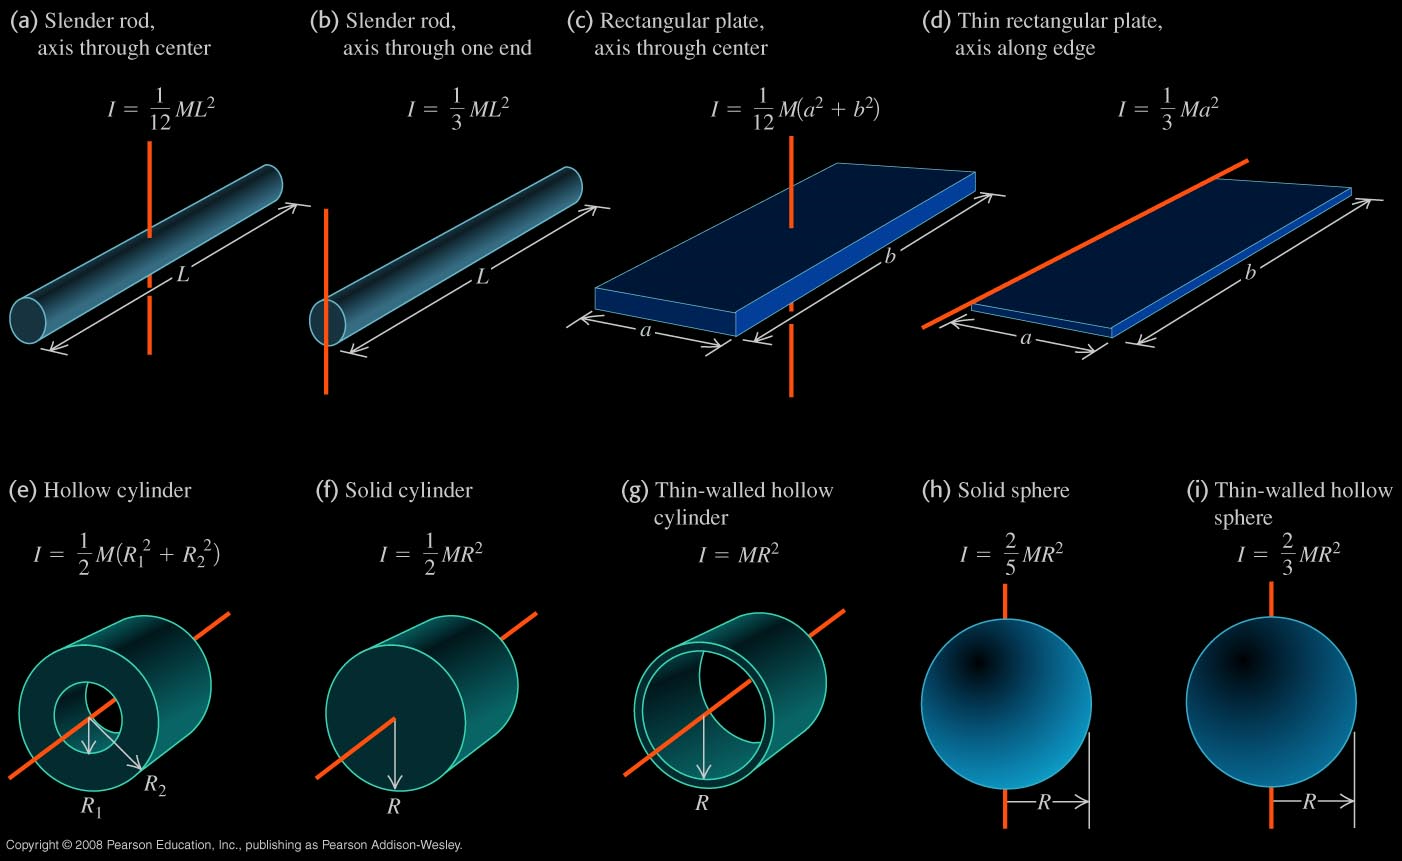
\includegraphics[width=\textwidth]{./rotational-inertia-table.png}
\end{figure}

\nvpx{20} \begin{equation}
	L = \rvec \times \pvec = mvr \sin \theta = mv\ell = I \omega
\end{equation}

\begin{equation}
	\hpx{36} L_0 = L_1 ~~~~ (\textrm{assuming no external torque})
\end{equation}

% \begin{equation}
% 	\Omega = \dot \phi = \dfrac \tau L = \dfrac{w r} {I \omega} ~~~~~ (\textrm{gyroscope})
% \end{equation}

% \begin{equation}
% 	\tau = \rvec_\cm \times \wvec
% \end{equation}

\ifx \combinedDocuments \undefined
\end{document}
\fi